\documentclass{article}
\usepackage[a4paper,left=3cm, right=3cm, top=2cm, bottom=2cm]{geometry}
\usepackage{amsmath}
\usepackage{graphicx}
\usepackage{caption}
\usepackage{setspace}
\usepackage{xcolor}
\usepackage{titlesec}
\usepackage{amssymb}
\usepackage{tcolorbox}
\usepackage{wrapfig}

\graphicspath{{graph/}}
\title{11.2 Series}
\date{}
\author{}
\setstretch{1.3} 

% \subsection* 형식 지정 (번호 없음)
\titleformat{name=\section, numberless}
  {\normalfont\large\bfseries\color{blue}}
  {}
  {0pt}
  {}
\geometry{a4paper, margin=1in}

\begin{document}
\maketitle

If we try to add the terms of an infinite sequence \(\{a_n\}_{n=1}^\infty\), we get an expression of the form
\[ a_1 + a_2 + a_3 + \cdots + a_n + \cdots \]
which is called an \textbf{infinite series} (or just a \textbf{series}) and is denoted by the symbol
\[ \sum_{n=1}^{\infty} a_n \quad \text{or} \quad \sum a_n \]

\section*{Partial Sums}
Let's consider the partial sums:
\begin{align*}
s_1 &= a_1 \\
s_2 &= a_1 + a_2 \\
s_3 &= a_1 + a_2 + a_3 \\
s_n &= \sum_{i=1}^{n} a_i = a_1 + a_2 + \cdots + a_n
\end{align*}
These partial sums form a new sequence \(\{s_n\}\), which may or may not have a limit.

\begin{tcolorbox}[
    colback=white,
    colframe=orange!80!white,
    title=Definition of a Convergent Series,
    boxrule=0.5mm,
    arc=3mm
    ]
    Given a series \( \sum_{n=1}^{\infty} a_n \), let \(s_n\) denote its nth partial sum. If the sequence of partial sums \(\{s_n\}\) is convergent and \( \lim_{n\to\infty} s_n = s \) exists as a real number, then the series \( \sum a_n \) is called \textbf{convergent} and we write:
    \[ \sum_{n=1}^{\infty} a_n = s \]
    The number \(s\) is called the \textbf{sum} of the series. If the sequence \(\{s_n\}\) is divergent, then the series is called \textbf{divergent}.
\end{tcolorbox}

\subsection*{EXAMPLE 1}
Suppose we know that the sum of the first \(n\) terms of the series \( \sum a_n \) is \( s_n = \dfrac{2n}{3n+5} \). Then the sum of the series is the limit of the sequence of partial sums:
\[ \sum_{n=1}^{\infty} a_n = \lim_{n\to\infty} s_n = \lim_{n\to\infty} \dfrac{2n}{3n+5} = \lim_{n\to\infty} \dfrac{2}{3+5/n} = \dfrac{2}{3} \]

\subsection*{EXAMPLE 2 (Telescoping Sum)}
Show that the series \( \sum_{n=1}^{\infty} \dfrac{1}{n(n+1)} \) is convergent, and find its sum.\\
\textbf{SOLUTION:}
Using partial fraction decomposition, we have \( a_n = \dfrac{1}{n(n+1)} = \dfrac{1}{n} - \dfrac{1}{n+1} \).
The nth partial sum is:
\[ s_n = \sum_{i=1}^{n} \left(\dfrac{1}{i} - \dfrac{1}{i+1}\right) = \left(1 - \dfrac{1}{2}\right) + \left(\dfrac{1}{2} - \dfrac{1}{3}\right) + \cdots + \left(\dfrac{1}{n} - \dfrac{1}{n+1}\right) = 1 - \dfrac{1}{n+1} \]
Thus, the sum of the series is:
\[ \lim_{n\to\infty} s_n = \lim_{n\to\infty} \left(1 - \dfrac{1}{n+1}\right) = 1 \]
The series converges to 1.
\begin{figure}[htbp]
    \centering
    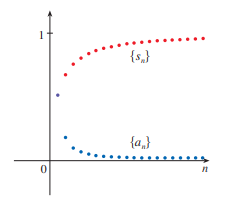
\includegraphics[width=0.35\textwidth]{graph73.png}
\end{figure}

\section*{Geometric Series}
A \textbf{geometric series} is a series of the form:
\[ a + ar + ar^2 + ar^3 + \cdots = \sum_{n=1}^{\infty} ar^{n-1}, \quad a \neq 0 \]
where \(r\) is the \textbf{common ratio.}

\begin{tcolorbox}[
    colback=white,
    colframe=orange!80!white,
    title=Sum of a Geometric Series,
    boxrule=0.5mm,
    arc=3mm
    ]
    The geometric series \( \sum_{n=1}^{\infty} ar^{n-1} \) is convergent if \(|r|<1\) and its sum is:
    \[ \sum_{n=1}^{\infty} ar^{n-1} = \dfrac{a}{1 - r}, \quad |r| < 1 \]
    If \(|r| \ge 1\), the geometric series is divergent.
\end{tcolorbox}

\subsection*{EXAMPLE 3}
Find the sum of the geometric series \( 5 - \dfrac{10}{3} + \dfrac{20}{9} - \dfrac{40}{27} + \cdots \).\\
\textbf{SOLUTION:}
The first term is \(a = 5\) and the common ratio is \(r = -\dfrac{2}{3}\). Since \(|r| = \dfrac{2}{3} < 1\), the series is convergent. The sum is:
\[ s = \dfrac{5}{1 - (-\frac{2}{3})} = \dfrac{5}{1 + \frac{2}{3}} = \dfrac{5}{5/3} = 3 \]
\begin{figure}[htbp]
    \centering
    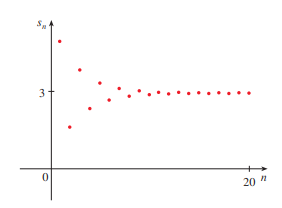
\includegraphics[width=0.35\textwidth]{graph72.png}
\end{figure}

\subsection*{EXAMPLE 4}
Is the series \( \sum_{n=1}^{\infty} 2^{2n} 3^{1-n} \) convergent or divergent?\\
\textbf{SOLUTION:}
Let's rewrite the nth term of the series in the form \(ar^{n-1}\):
\[ a_n = 2^{2n} 3^{1-n} = (2^2)^n 3^{-(n-1)} = 4^n \dfrac{1}{3^{n-1}} = 4 \cdot \dfrac{4^{n-1}}{3^{n-1}} = 4 \left( \dfrac{4}{3} \right)^{n-1} \]
This is a geometric series with \(a=4\) and common ratio \(r = 4/3\). Since \(r > 1\), the series \textbf{diverges}.

\subsection*{EXAMPLE 5}
For what values of \(x\) does the series \( \sum_{n=0}^{\infty} x^n \) converge?\\
\textbf{SOLUTION:}
This is a geometric series with \(a=1\) and \(r=x\). It converges when \(|x|<1\), that is, for \(-1 < x < 1\). The sum is \(\dfrac{1}{1-x}\).

\subsection*{EXAMPLE 6}
Write the number \(2.3\overline{17} = 2.3171717\dots\) as a ratio of integers.\\
\textbf{SOLUTION:}
\[ 2.3\overline{17} = 2.3 + \dfrac{17}{10^3} + \dfrac{17}{10^5} + \dfrac{17}{10^7} + \cdots \]
This contains a geometric series with first term \(a = \dfrac{17}{1000}\) and common ratio \(r = \dfrac{1}{100}\).
\[ 2.3\overline{17} = 2.3 + \dfrac{\frac{17}{1000}}{1 - \frac{1}{100}} = \dfrac{23}{10} + \dfrac{\frac{17}{1000}}{\frac{99}{100}} = \dfrac{23}{10} + \dfrac{17}{1000} \cdot \dfrac{100}{99} = \dfrac{23}{10} + \dfrac{17}{990} \]
\[ = \dfrac{23 \cdot 99 + 17}{990} = \dfrac{2277 + 17}{990} = \dfrac{2294}{990} = \dfrac{1147}{495} \]

\subsection*{EXAMPLE 7}
Find the sum of the series \( \sum_{n=0}^{\infty} x^n \), where \(|x|<1\).\\
\textbf{SOLUTION:}
This is a geometric series with \(a=1\) and ratio \(r=x\). Since \(|x|<1\), it converges and the sum is:
\[ \sum_{n=0}^{\infty} x^n = \dfrac{1}{1-x} \]


\subsection*{EXAMPLE 8 (The Harmonic Series)}
The series \( \sum_{n=1}^{\infty} \dfrac{1}{n} = 1 + \dfrac{1}{2} + \dfrac{1}{3} + \dfrac{1}{4} + \cdots \) is called the \textbf{harmonic series} and is divergent.\\
\textbf{SOLUTION:}
We show this by looking at the partial sums.
\[ s_1 = 1, \quad s_2 = 1.5, \quad s_4 = s_2 + \dfrac{1}{3} + \dfrac{1}{4} > 1.5 + \dfrac{1}{4} + \dfrac{1}{4} = 2 \]
\[ s_8 = s_4 + \dfrac{1}{5} + \dfrac{1}{6} + \dfrac{1}{7} + \dfrac{1}{8} > 2 + 4 \cdot \dfrac{1}{8} = 2.5 \]
In general, one can show that \(s_{2^n} > 1 + n/2\). This shows that \(s_n \to \infty\) as \(n \to \infty\), so the harmonic series diverges.

\begin{tcolorbox}[
    colback=white,
    colframe=orange!80!white,
    title=Theorem: Test for Divergence,
    boxrule=0.5mm,
    arc=3mm
    ]
    If \( \lim_{n\to\infty} a_n \) does not exist or if \( \lim_{n\to\infty} a_n \neq 0 \), then the series \( \sum_{n=1}^{\infty} a_n \) is divergent.
\end{tcolorbox}
\textbf{Note:} If \( \lim_{n\to\infty} a_n = 0 \), we cannot conclude that the series converges.

\subsection*{EXAMPLE 9}
Show that the series \( \sum_{n=1}^{\infty} \dfrac{n^2}{5n^2+4} \) diverges.\\
\textbf{SOLUTION:}
\[ \lim_{n\to\infty} a_n = \lim_{n\to\infty} \dfrac{n^2}{5n^2+4} = \lim_{n\to\infty} \dfrac{1}{5+4/n^2} = \dfrac{1}{5} \neq 0 \]
Since the limit is not 0, the series diverges by the Test for Divergence.

\begin{tcolorbox}[
    colback=white,
    colframe=orange!80!white,
    title=Properties of Convergent Series,
    boxrule=0.5mm,
    arc=3mm
    ]
    If \( \sum a_n \) and \( \sum b_n \) are convergent series and \(c\) is a constant, then:
    \begin{itemize}
        \item[(i)] \( \sum_{n=1}^{\infty} c a_n = c \sum_{n=1}^{\infty} a_n \)
        \item[(ii)] \( \sum_{n=1}^{\infty} (a_n + b_n) = \sum_{n=1}^{\infty} a_n + \sum_{n=1}^{\infty} b_n \)
        \item[(iii)] \( \sum_{n=1}^{\infty} (a_n - b_n) = \sum_{n=1}^{\infty} a_n - \sum_{n=1}^{\infty} b_n \)
    \end{itemize}
\end{tcolorbox}

\subsection*{EXAMPLE 10}
Find the sum of the series \( \sum_{n=1}^{\infty} \left( \dfrac{3}{n(n+1)} + \dfrac{1}{2^n} \right) \).\\
\textbf{SOLUTION:}
The series \( \sum 1/2^n \) is a geometric series with \(a=1/2\) and \(r=1/2\), so its sum is \( S = \dfrac{1/2}{1-1/2} = 1 \).
From Example 2, we know \( \sum \dfrac{1}{n(n+1)} = 1 \).
Therefore, the given series converges and its sum is:
\[ \sum_{n=1}^{\infty} \left( \dfrac{3}{n(n+1)} + \dfrac{1}{2^n} \right) = 3 \sum_{n=1}^{\infty} \dfrac{1}{n(n+1)} + \sum_{n=1}^{\infty} \dfrac{1}{2^n} = 3(1) + 1 = 4 \]\\\\

\textbf{Note:}
A finite number of terms does not affect the convergence or divergence of a series. For instance, suppose that we were able to show that the series
$\sum_{n=4}^{\infty} \dfrac{n}{n^3 + 1} $
is convergent. \\
Since $\sum_{n=1}^{\infty} \dfrac{n}{n^3 + 1} = \dfrac{1}{2} + \dfrac{2}{9} + \dfrac{3}{28} + \sum_{n=4}^{\infty} \dfrac{n}{n^3 + 1}$
it follows that the entire series \( \sum_{n=1}^{\infty} \dfrac{n}{n^3 + 1} \) is convergent.\\
Similarly, if it is known that the series \( \sum_{n=N+1}^{\infty} a_n \) converges, then the full series
$\sum_{n=1}^{\infty} a_n = \sum_{n=1}^{N} a_n + \sum_{n=N+1}^{\infty} a_n $
is also convergent.
\end{document}